\section{12.1 Wady metod bezpośrednich}

\begin{frame}{Wady metod bezpośrednich}
  \begin{block}{\textbf{Złożoność obliczeniowa} ${\sim}N^3$}
    \begin{itemize}
      \item{ $M=\frac{1}{3}n^3+n^2-\frac{1}{3}n$ ($*$,$/$)}
      \item{ $D=\frac{1}{3}n^3+\frac{1}{2}n^2-\frac{5}{6}n$ ($+$)}
    \end{itemize}
    Np. $10^4$ punktów siatki przestrzennej (mesh points)
    \begin{itemize}
      \item{100 x 100   (2 -- D)}
      \item{20 x 20 x 20   (3 -- D)}
      \item{metoda eliminacji Gaussa to $\sim 10^{12}$ operacji}
      \item{1 operacja trwa $\sim 10^{-8}$ s.}
      \item{$10^4$ czyli $\sim$ 3 godziny}
    \end{itemize}
  \end{block}
\end{frame}

\begin{frame}{}
  \begin{block}{\textbf{Zwykle}}
    \begin{itemize}
      \item{czas symulacji $\sim$ 1h,}
      \item{ilość kroków czasowych $\sim$ 1000,}
      \item{cały krok - to rozwiązywanie układu równań,}
      \item{1 operacja $\sim 10^{-8}$ s,}
      \item{il. punktów siatki $\sim 10^4$ ($\equiv$ ilość równań)}
    \end{itemize}
  \end{block}
\end{frame}

\begin{frame}{}
  \begin{block}{\textbf{Potrzebne są metody o znacznie mniejszej złożoności}}
    Metody takie powinny być oparte na własnościach r.r. cząstkowych (zwykle - źródła równań liniowych):
    \begin{itemize}
      \item{liniowość,}
      \item{wymiar,}
      \item{możliwości separacji zmiennych,}
      \item{zakres zmian współczynników,}
      \item{kształt geometryczny obszaru,}
      \item{warunki brzegowe - postać.}
    \end{itemize}
  \end{block}
\end{frame}

\begin{frame}{}
  \textbf{Metody bezpośrednie zaburzają strukturę macierzy rzadkich}
  \newline 2 - D $\rightarrow$ operator 5-cio punktowy
  \begin{figure}
    \centering
    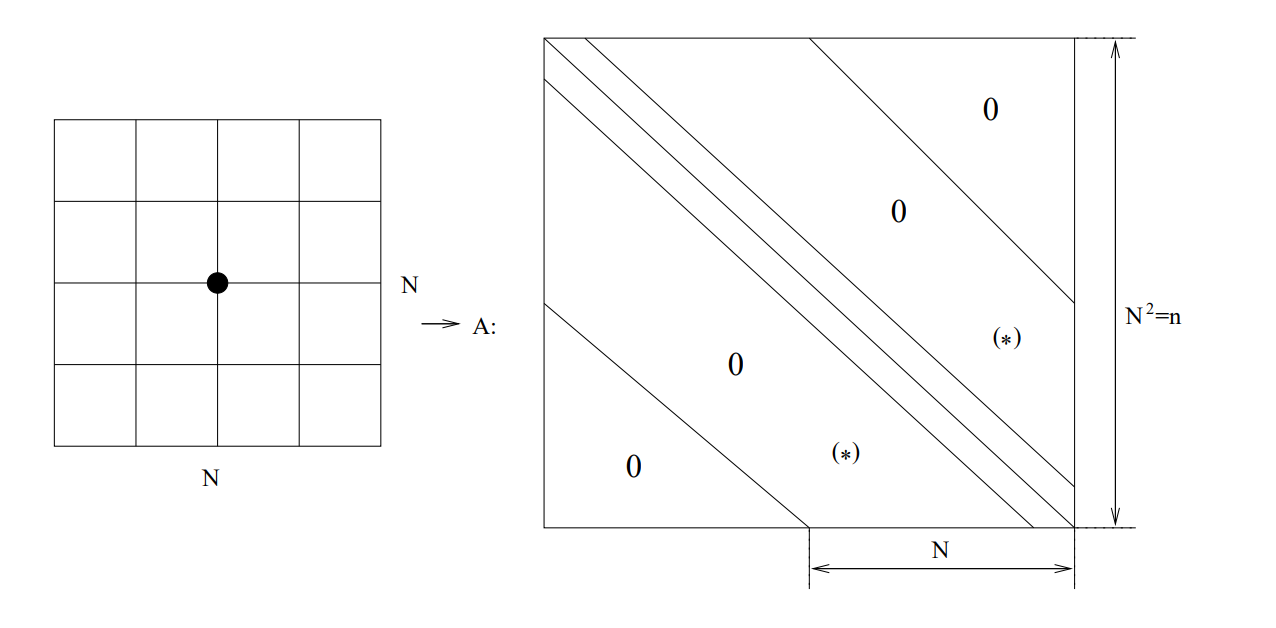
\includegraphics[height=0.5\textheight, width=0.8\textwidth]{img/12/iteracja1}
  \end{figure}
\end{frame}

\begin{frame}{}
  \begin{block}{\textbf{Metody bezpośrednie zaburzają strukturę macierzy rzadkich}}
    \begin{itemize}
      \item{$\sim 5*N^2$ współczynników $\neq$ 0}
      \item{ale: po zastosowaniu metody eliminacji Gaussa znikają zera z wstęg
      \newline (*) $\rightarrow$ trzeba wtedy pamiętać $2*N^3$ współczynników}
      \item{Macierz wstęgowa: $m_{ij}=0$ dla $|i-j|>k$}
      \item W mmetodach polegających na mnożeniu $A*x^{(t)}$ w kroku t zamiast $n^2 \rightarrow k*n$ mnożeń $\Rightarrow$ wtedy łatwo o:
      \begin{center}
      $s*k*n<n^3$
      \end{center}
      \item gdzie s - ilość kroków, a $n^3$ - złożoność metod bezpośrednich.
    \end{itemize}
  \end{block}
\end{frame}
